\section{Dual-Debate Decision Validation}\label{sec:debate}

Financial trading decisions are inherently adversarial: every buyer believes an asset will rise, while every seller believes it will fall. Automated systems that lack adversarial scrutiny can suffer from confirmation bias, overfitting to bullish signals, or simply failing to consider contrarian scenarios. PolyEdge addresses this risk through a dual-debate validation system called MiroFish, which enforces structured adversarial argumentation before capital deployment. The system is inspired by the AI safety via debate framework \citep{irving2018ai} and the critique-revision approach of Constitutional AI \citep{bai2022constitutional}, adapted for financial signal validation.

\subsection{Debate Architecture}

The debate system is composed of three agent roles (see Figure~\ref{fig:debate_flow}):

\begin{enumerate}
    \item \textbf{Bull Agent.} An LLM prompt tuned for optimistic reasoning. Given a \texttt{TradingSignal}, the Bull agent generates arguments in favor of the trade: citing price momentum, favorable probabilities, market sentiment, whale activity, or macroeconomic indicators.
    \item \textbf{Bear Agent.} An LLM prompt tuned for pessimistic reasoning. The Bear agent generates arguments against the trade: citing mean reversion, liquidity constraints, model miscalibration, recent losses, or structural market risks.
    \item \textbf{Judge Agent.} An LLM prompt tuned for neutral evaluation. The Judge receives both the Bull and Bear arguments, along with the raw signal metadata (confidence, edge, market ticker, time of day, recent P\&L of the strategy). It produces a \texttt{DebateVerdict} with a categorical decision (\texttt{APPROVE}, \texttt{REJECT}, or \texttt{DEFER}) and a continuous confidence score.
\end{enumerate}

The three agents are served by the same LLM provider ensemble used for signal generation (Claude and Groq), ensuring that debate quality scales with the underlying model capabilities. The agents operate with different system messages and temperature settings: Bull at 0.9 (creative, exploratory), Bear at 0.9 (creative contrarian), and Judge at 0.1 (conservative, fact-based).

\subsection{Verdict Routing and Thresholds}

After the Judge renders its verdict, the system applies configurable thresholds:
\begin{itemize}
    \item \textbf{Confidence $>$ 0.70.} The signal is automatically approved and forwarded to execution.
    \item \textbf{Confidence 0.40--0.70.} The signal is queued for manual review on the dashboard. A human operator can approve or reject it.
    \item \textbf{Confidence $<$ 0.40.} The signal is automatically rejected. The rejection reason (including the Bear agent's primary objection) is logged.
\end{itemize}

These thresholds are adjustable per risk profile and per market category. For example, low-liquidity political markets may use a higher approval threshold (0.80) than high-volume crypto markets (0.65), reflecting the different risk profiles of each asset class.

\subsection{TradeAttempt Ledger}

Every signal that enters the debate system, regardless of outcome, is recorded in the \texttt{TradeAttempt} ledger \citep{nygard2018release}. Each ledger entry contains:
\begin{itemize}
    \item Signal source (strategy name, genome ID, timestamp);
    \item Bull argument text (truncated to 500 tokens);
    \item Bear argument text (truncated to 500 tokens);
    \item Judge verdict and confidence score;
    \item Execution result (executed, rejected, deferred) and final P\&L (if executed);
    \item Rejection reason (if rejected);
    \item Time elapsed in debate (to monitor latency).
\end{itemize}

The ledger serves three purposes: (1) post-hoc auditability for debugging and compliance, (2) calibration monitoring (comparing Judge confidence to actual outcomes), and (3) training data for improving the Judge model over time. The dashboard renders the ledger as a ``Control Room'' view where operators can inspect the debate history of any trade.

\subsection{Fallback Mechanism}

The MiroFish debate system relies on external LLM API calls, which can fail due to rate limits, network outages, or provider unavailability. When the external service returns a 5xx status code or times out (default: 30 seconds), the system falls back to a local debate engine. The local engine uses the same Bull/Bear/Judge prompt templates but sends them to the locally configured LLM provider (Claude or Groq via the standard AI client). This ensures that debate validation never blocks signal flow entirely. The fallback event is logged in the TradeAttempt ledger with \texttt{source=\"local\_fallback\"} for audit purposes.

\subsection{Integration with Risk Management}

The debate system operates \emph{after} risk validation and \emph{before} execution. The signal flow is therefore:

\begin{center}
\texttt{TradingSignal} $\rightarrow$ \texttt{RiskManager.validate()} $\rightarrow$ \texttt{MiroFish.debate()} $\rightarrow$ \texttt{strategy\_executor.execute()}
\end{center}

This ordering is intentional: risk validation filters out signals that violate capital-protection rules (size, exposure, drawdown), while debate validation filters out signals that lack adversarial support. A signal can pass risk but fail debate, or vice versa. The separation of concerns ensures that neither system develops blind spots: risk management enforces hard numerical constraints, while debate validation enforces qualitative reasoning.

\subsection{Dashboard Arena}

The frontend provides a real-time ``Arena'' view that displays the current debate state: Bull text on the left, Bear text on the right, and the Judge verdict in the center with a confidence bar. The Arena updates via Server-Sent Events as new signals enter the debate system. Operators can click on any signal to view the full argument text, the signal metadata, and the execution decision. This human-in-the-loop interface is particularly valuable during the paper-trading phase, where operators can validate that the debate system is making reasonable decisions before enabling auto-approval.

\begin{figure}[H]
    \centering
    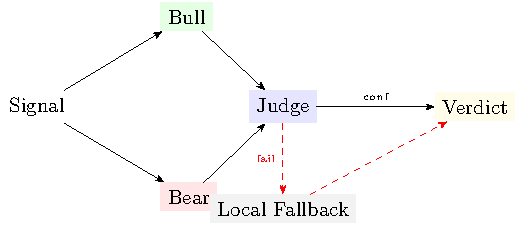
\includegraphics[width=0.95\textwidth]{figures/debate_flow.pdf}
    \caption{MiroFish dual-debate signal validation flow. Trading signals are routed to Bull and Bear debate agents. A Judge agent evaluates arguments and generates a verdict with confidence score. Failed signals fallback to a local debate engine before rejection.}
    \label{fig:debate_flow}
\end{figure}

The dual-debate system is not a novel contribution in the abstract sense: adversarial validation and ensemble judgment are well-established in AI safety \citep{irving2018ai, bai2022constitutional}. Our contribution is the operationalization of these principles in a live financial system, with hard latency budgets, fallback mechanisms, and persistent audit trails. To our knowledge, no prior prediction-market trading system has integrated structured adversarial debate into its signal-validation pipeline.
